\twocolumn[
\begin{center}
\title{\color[cmyk]{1, 0.57, 0, 0.38}{\Huge\bfseries Intervista a: Gianluca Sforna\\}} % definisco il titolo dell'articolo
\author{\scriptsize Gabriele Trombini (mailga@fedoraonline.it)} % definisco l'autore e altre informazioni
\date{}
\maketitle
\normalsize
\hfill
\end{center}
{\color[cmyk]{1, 0.46, 0, 0}\LARGE Le interviste di Folio - incontriamo Gianluca Sforna}  \\
\small\sl Abbiamo chiesto al nostro amico Gianluca di rispondere a 10 domande, sperando anche di metterlo in difficoltà. La qualità delle risposte non ci ha affatto sorpreso.\\
]
\begin{figure}[htbp]
\centering
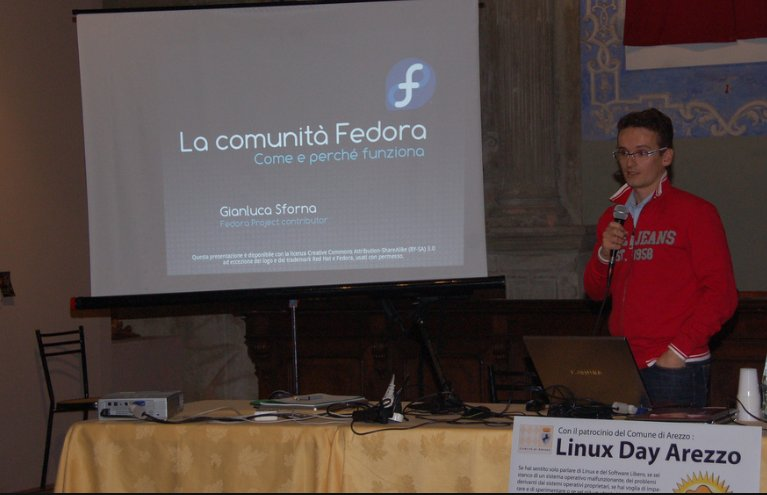
\includegraphics[scale=.35]{articoli/varie/immagini/giallu.jpg}\\
\end{figure}
\singlespacing
\definecolor{shadecolor}{cmyk}{0, 0, 0, 0.1}
\begin{shaded}
{\footnotesize
\color[cmyk]{1, 0.57, 0, 0.38}
\emph{Chi è \textbf{Gianluca Sforna? (@giallu)}\\
classe 1972, programmatore e sysadmin.\\
Inizia a lavorare stabilmente su Linux nel 1999 con Red Hat Linux 6.0;
nel 2003 diventa prima utente e poi contributor del progetto Fedora.\\
Oggi è maintainer di diversi pacchetti RPM ospitati tra repository
ufficiali (Fedora, RPMFusion) e privati, traduttore ed ambassador del
progetto.\\ Il suo blog: \\http://morefedora.blogspot.com}
}
\end{shaded}
\bigskip
\onehalfspacing
\emph{\textbf{FOL: 1) chi è il Fedora Project?}}\\
\emph{\textbf{Giallu: }}Il progetto non è nessuno in particolare, ma in effetti si può dire che tutti i partecipanti al progetto in qualche modo sono Fedora: infatti anche il più piccolo dei contributi permette al progetto e agli altri partecipanti di crescere e migliorarsi, quindi il progetto nel suo complesso si può sicuramente considerare ``figlio'' di ogni contributor. Non a caso ho partecipato ad EuroPython 2011 con questo badge:
\begin{figure}[htbp]
\centering
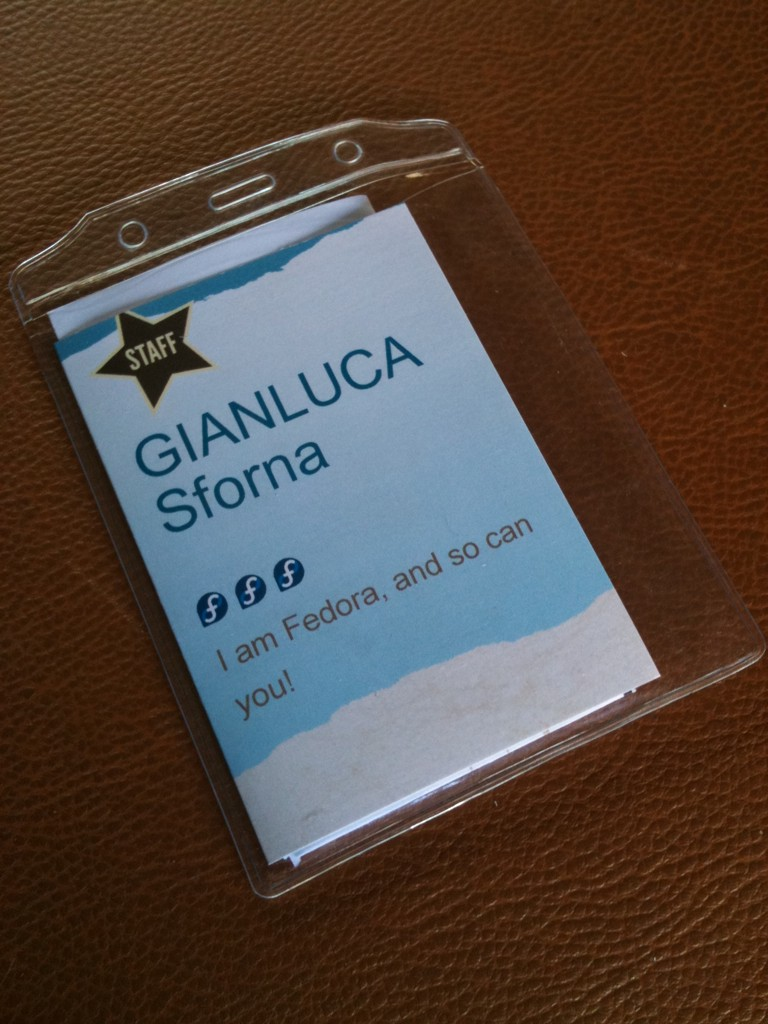
\includegraphics[scale=.10]{articoli/varie/immagini/badge.jpg}\\
\end{figure} \\

\emph{\textbf{FOL: 2) gli ambassador promuovono il progetto o il sistema operativo?}}\\
\emph{\textbf{Giallu: }}Direi entrambi: gli Ambassador promuovono senz'altro il progetto e i suoi valori, ma è chiaro che la distribuzione era e rimane il prodotto principale e più visibile quindi trovo difficile che si possa scindere i due aspetti.\\

\emph{\textbf{FOL: 3) sbaglia qualcosa, il Fedora Project? Se sbaglia, in che modo?}}\\
\emph{\textbf{Giallu: }}Un progetto così grande sicuramente ha sia punti di forza che debolezze. E' però praticamente impossibile dare un giudizio assoluto, visto che tutto dipende da cosa si usa come metro per definirne il successo. Se per dire mi aspetto dal progetto una distribuzione che posso installare su un server  e supportare per una decina di anni, troverò che si stanno compiendo molti errori. Lo stesso se mi aspetto una distribuzione ``rolling'', che includa sempre e comunque solo le ultime versioni di ogni software. 
Da notare che gli obiettivi del progetto non sono ``statici'' ma sono stati più volte sviluppati, raffinati e chiariti; ad oggi, se esaminiamo la pagina del wiki che li elenca (https://fedoraproject.org/\\wiki/Objectives) direi che il progetto nel suo complesso è decisamente sulla buona strada.\\

\emph{\textbf{FOL: 4) cosa rubereste a Debian, a Slackware ed a gentoo?}}\\
\emph{\textbf{Giallu: }}Premesso che dopo tanti anni di uso esclusivo di Fedora (e derivate) non conosco bene la situazione dei nostri ``cugini'', devo dire che di Debian ammiro l'organizzazione complessiva che riesce a "tenere" un gran numero di utenti e sviluppatori anche a dispetto dei loro ingombranti vicini di casa.\\

\emph{\textbf{FOL: 5) non vi pare che i linux day e i Fudcon siano eventi riservati ad una ristretta utenza, in fondo si riferiscono sempre agli stessi ambienti?}}\\
\emph{\textbf{Giallu: }}Credo che i due eventi siano profondamente diversi: se i Linux Day si rivolgono ad una ampia platea essendo un evento divulgativo per definizione (anche se poi sono tanti i partecipanti già introdotti alla filosofia del software libero), il FUDCon mi sembra più un evento del "fare" e per questo sicuramente ricco di utenti avanzati e sviluppatori che approfittano della occasione di aggregazione per accelerare quelle attività di sviluppo a volte rallentate dalla distanza fisica tra i contributor. Concordo comunque sul fatto che siano eventi di ``nicchia'', visto che comunque ancora oggi, a dispetto di tutti i progressi fatti, Linux continua ad essere il settore ``Altro'' vicino a ``Windows'' e ``MacOSX'' dei diagrammi a torta.\\

\emph{\textbf{FOL: 6) dove pensate che si possa essere più incisivi nella promozione?}}\\
\emph{\textbf{Giallu: }}Direi un po' ovunque: scuole, università, LUG, eventi, aziende pubbliche private etc. 
Ad oggi mi pare evidente che altre distribuzioni siano riuscite ad attrarre un grosso numero di utenti (che è comunque un bene visto che per lo più provengono da altri sistemi operativi). Se consideriamo che Fedora si rivolge ad un pubblico più consapevole la situazione non è drammatica, ma siccome penso sia più difficile ``convertire'' un utente piuttosto che acquisirlo la prima volta, spero che lo sforzo di marketing sul progetto sia sempre più efficace.\\

\emph{\textbf{FOL: 7) perchè l'utente dovrebbe usare fedora e non altre distro? solo per il free software, non vi pare un po' troppo idealistico?}}\\
\emph{\textbf{Giallu: }}Il software libero l'utente lo trova in tutte le distro; non tutte però ti garantiscono che la totalità dei contenuti siano effettivamente ridistribuibili; per dire, se sei una azienda ed hai intenzione di produrre e vendere un prodotto hardware o software basato su Linux, Fedora può essere una ottima scelta proprio per questo motivo. La altre motivazioni si trovano nella metodologia di sviluppo: collaborazione con gli upstream (i progetti su cui si basa la distribuzione tipo kernel, GNOME, KDE, etc), aggiornamenti rapidi (siamo quasi sempre i primi a fornire le ultime versioni disponibili), totalità degli strumenti usati disponibili (per cui chiunque può farsi la ``sua'' distribuzione derivata)
L'utente comune tende invece a dare valore ad altre caratteristiche, ad esempio che i suoi mp3 o DVD si possano riprodurre semplicemente cliccandoci sopra (per inciso, questa cosa funziona proprio in questo modo in Fedora, previa attivazione dei repository RPMFusion) oppure che la esistenza di driver proprietari venga notificata automatizzandone l'installazione.
Purtroppo questo a volte si scontra con il fatto che Fedora punta alla produzione e integrazione del migliore e più recente software libero: per esempio, molto spesso nel passato i driver ATI disponibili erano incompatibili con il server X o con il kernel distribuiti in quel momento da Fedora, e solo con mesi di ritardo AMD ha provveduto a fornire driver funzionanti; in queste condizioni non c'è molto che il progetto possa fare, se non lavorare ancora di più per rendere inutili tali driver, sostituiti dalle loro controparti open.\\

\emph{\textbf{FOL: 8) ritieni di aver fatto tutto il possibile per promuovere Fedora?}}\\
\emph{\textbf{Giallu: }}Sicuramente no:  il lavoro non manca mai, ma il tempo e l'energia a volte non sono facili da trovare. Per questo penso sia sempre prioritario trovare e motivare nuovi contributor, così che la riserva di idee e manodopera per nuove iniziative sia sempre alimentata.\\

\emph{\textbf{FOL: 9) Fedora avrà un ritorno dall'utenza italiana?}}\\
\emph{\textbf{Giallu: }}Sicuramente. La barriera alla partecipazione al progetto è sempre più bassa e chiunque, a prescindere dalle proprie capacità tecniche, può dare un contributo. Basta guardarsi un po' intorno per scoprire il team più adatto alle proprie inclinazioni e capacità ed iniziare!\\

\emph{\textbf{FOL: 10) Come siamo noi italiani rispetto alla totalità del progetto?}}\\
\emph{\textbf{Giallu: }}Ci sono team ben più organizzati, ma devo dire che gli Italiani nel progetto non mancano a tutti i livelli. Se solo trovassimo il modo di aumentarne la coesione credo che saremmo tra i gruppi più importanti del progetto...
\\
